The Finite Element Method (FEM) is by no means the only method 
to solve PDEs in geodynamics, nor is it necessarily the best one.
Other methods are employed very succesfully, such as the Finite Difference 
Method (FDM), the Finite Volume Method (FVM), and to a lesser extent
the Discrete Element Method (DEM) \cite{tasy05,egho07,egsc07,funi14}, 
or the Element Free Galerkin Method (EFGM) \cite{hans03}.
I have been using FEM since 2008 and I do not have real 
experience to speak of in FVM or FDM so I concentrate in this book 
on what I know best. 

%..............................................
\subsubsection{A bit of history for fun ... }

The first papers I could find showcasing the FEM in geodynamics are listed hereafter
(I arbitrarily stop at 1995):
\cite{gart78}, 
\cite{anbr80}\cite{mera80}
\cite{engl82}
\cite{thar85}
\cite{enho86}\cite{mofr86}
\cite{zupa86}
\cite{boww89}
\cite{brau94}
\cite{brbe95}.
I hereunder show a few plots taken from early geodynamics papers.

\begin{center}
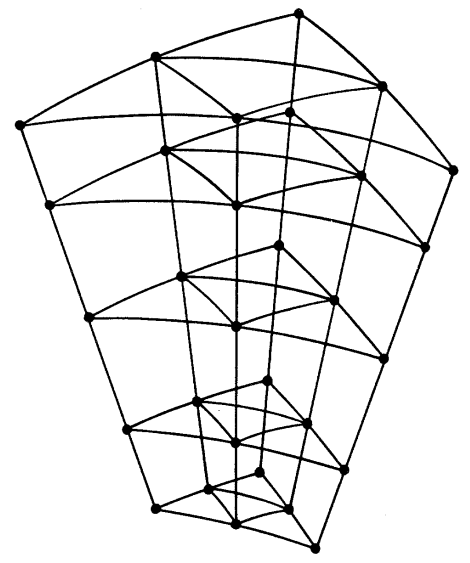
\includegraphics[height=4cm]{images/history/baum85a}
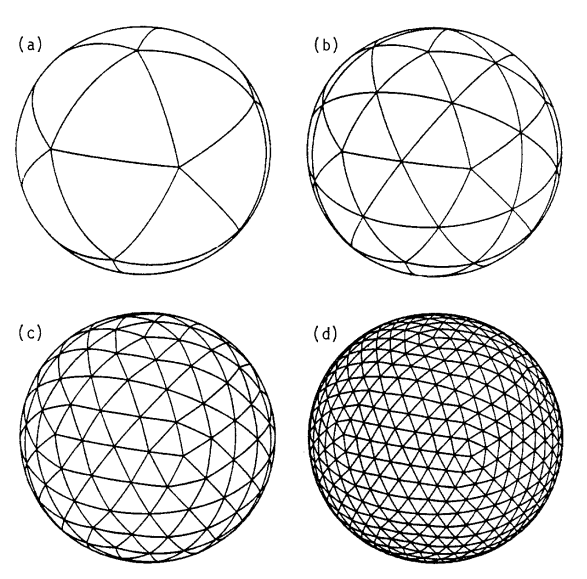
\includegraphics[height=4cm]{images/history/baum85b}\\
{\small 1985: Three-Dimensional Treatment of Convective Flow in the Earth's Mantle.
\cite{baum85}}
\end{center}

\begin{center}
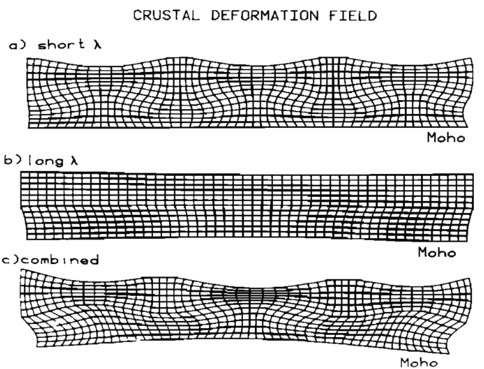
\includegraphics[width=7cm]{images/history/zupf86}\\
{\small 1986: Lithospheric necking: a dynamic model for rift morphology \cite{zupf86}}
\end{center}

\begin{center}
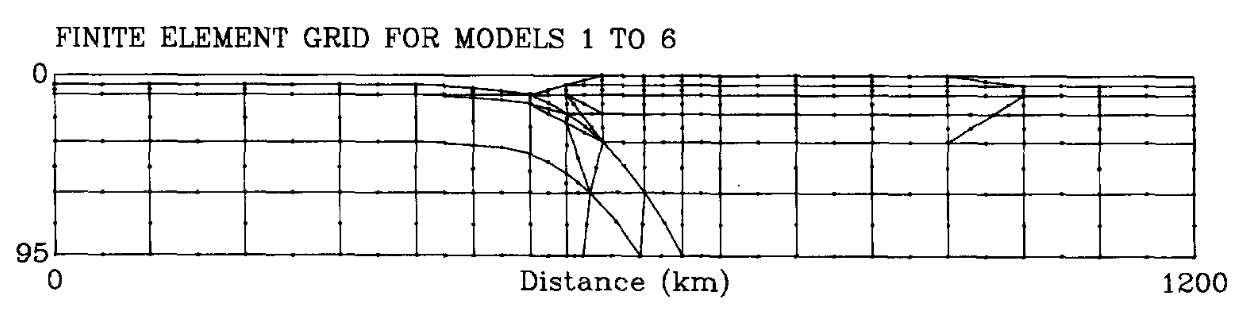
\includegraphics[width=7cm]{images/history/boww89}\\
{\small 1989: Plate boundary forces at subduction zones and trench-arc compression \cite{boww89}}
\end{center}

\begin{center}
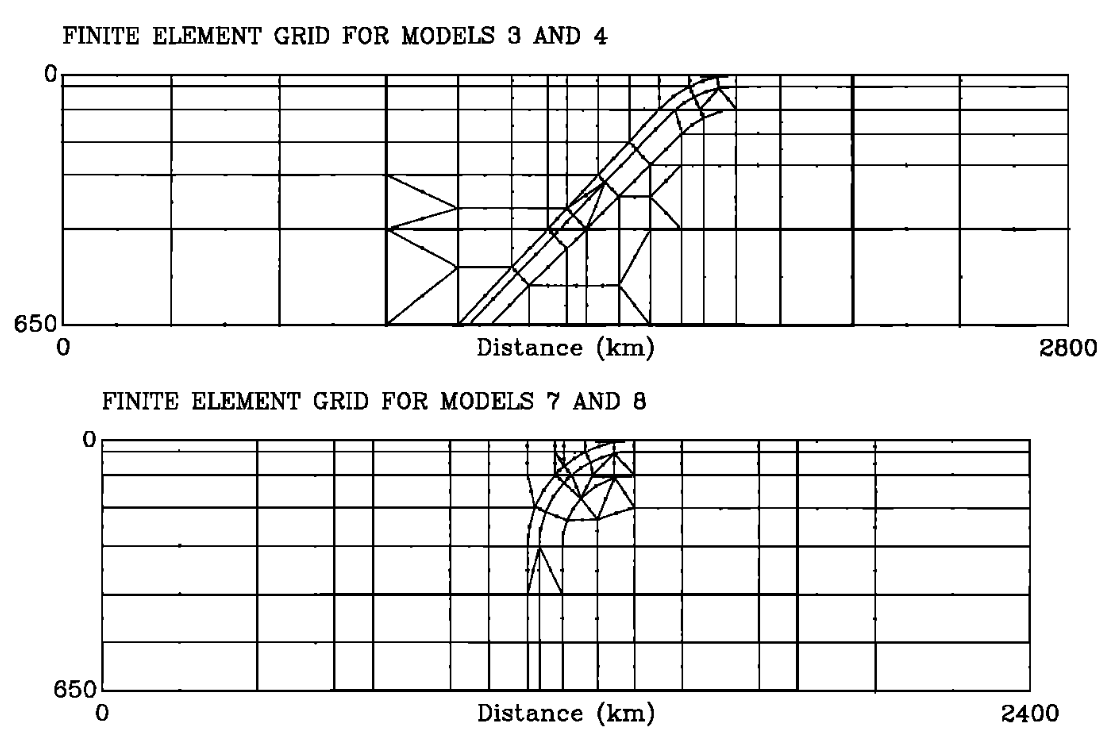
\includegraphics[width=7cm]{images/history/whbw92}\\
{\small 1992: Stresses and plate boundary forces associated with subduction plate margins
\cite{whbw92}}
\end{center}

\begin{center}
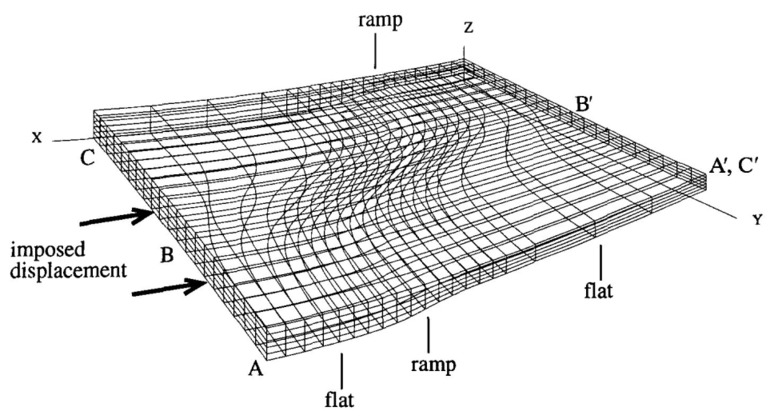
\includegraphics[width=7cm]{images/history/brau93}\\
{\small 1993: 3D numerical modeling of
compressional orogenies: Thrust geometry and
oblique convergence \cite{brau93}}
\end{center}

\begin{center}
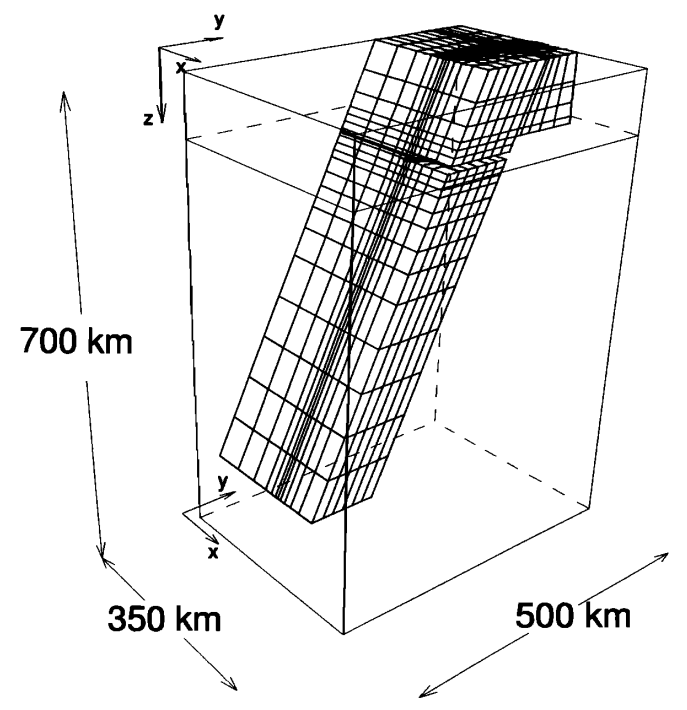
\includegraphics[height=5cm]{images/history/yowo95}\\
{\small 1995: 3D numerical modeling of detachment of subducted 
lithosphere \cite{yowo95}}
\end{center}

\begin{center}
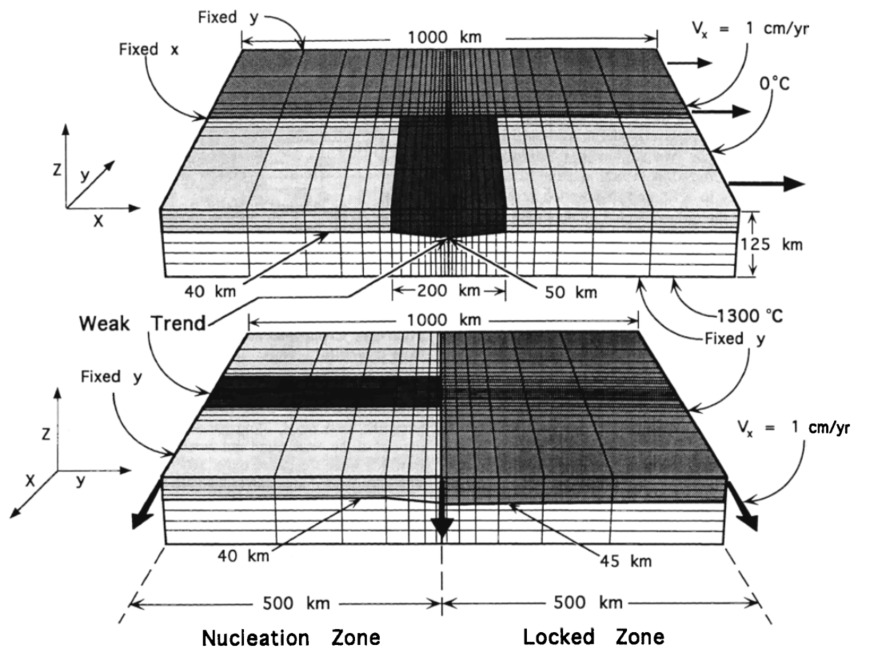
\includegraphics[height=6cm]{images/history/dusa96}\\
{\small 1996: 3D dynamical model of continental rift propagation and 
margin plateau formation \cite{dusa96}}
\end{center}

